\section{ R-A*mbush: Ambush with fixed radio R}

Getting agents to perform \ambush\ from the starting 
point can be disadvantageous, since they can take 
unnecessarily longer routes, when avoiding each other’s paths. 
Making the agents perform \ambush\ when they are closer
 to the goal could shorten the increment in this cost. 
 
With this reasoning as a base, \rambush\ is proposed.
 It is an A$^*$mbush modification that performs \astar until
the agent gets inside a fixed radius $R$ around the goal point.
Once at this stage, the agent stats performing \ambush. 
Note that this transition happens only once. Even if  the
\ambush\ algorithm makes the agent leave the radio area,
it will not start performing \astar again. This prevents a 
loop that the intelligence could easily fall into. First, the agent,
following the path given by A$^*$ comes inside the radius R,
then \ambush\ takes it out of the area when trying to go for 
a unexplored route, subsequently, this behaviour is interrupted 
and the A$^*$ method takes control again, making the agent go 
inside the radio. Those steps could be repeated infinitely, 
so once the radio $R$ is crossed, only \ambush\ behaviour takes place.
Figure \ref{fig:rambush} shows the performance of the \rambush\
algorithm.

\begin{figure}[htb]
	\centerline{
		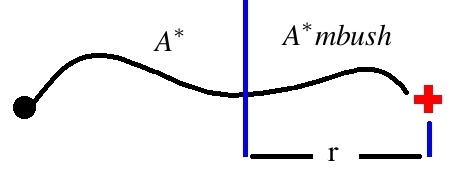
\includegraphics[width=0.48\columnwidth]{figures/rambush.jpg}
	}
	\caption{\label{fig:rambush}
	     R-A$^*$mbush. The agent located in the black point
	     tries to reach the cross.}
\end{figure}

The radius $R$ is measured in real distance (A$^*$). 
It was chosen over the Euclidean, because obstacles in games 
could make the agents take ambush routes when the path to 
get to the goal is still very long, and this would antagonize 
the purpose of reducing the path cost when possible.
